\documentclass[FM, Dis]{tulthesis}

\usepackage[czech, english]{babel}
\usepackage[utf8]{inputenc}

\DeclareUnicodeCharacter{00A0}{~}

\usepackage{amsmath}
\usepackage{amsfonts}
\usepackage{amssymb}
\usepackage{amsthm}
\usepackage{esint}
%
\newtheorem{theorem}{Theorem}[section]
\newtheorem{proposition}[theorem]{Proposition}
\newtheorem{definition}[theorem]{Definition}
\newtheorem{remark}[theorem]{Remark}
\newtheorem{lemma}[theorem]{Lemma}
\newtheorem{corollary}[theorem]{Corollary}
%\newtheorem{exercise}[theorem]{Cvičení}

%\numberwithin{equation}{document}
%
\def\div{{\rm div}}
\def\Lapl{\Delta}
\def\grad{\nabla}
\def\supp{{\rm supp}}
\def\dist{{\rm dist}}
%\def\chset{\mathbbm{1}}
\def\chset{1}
%
\def\Tr{{\rm Tr}}
\def\to{\rightarrow}
\def\weakto{\rightharpoonup}
\def\imbed{\hookrightarrow}
\def\cimbed{\subset\subset}
\def\range{{\mathcal R}}
\def\leprox{\lesssim}
\def\argdot{{\hspace{0.18em}\cdot\hspace{0.18em}}}
\def\Distr{{\mathcal D}}
\def\calK{{\mathcal K}}
\def\FromTo{|\rightarrow}
\def\convol{\star}
\def\impl{\Rightarrow}
\DeclareMathOperator*{\esslim}{esslim}
\DeclareMathOperator*{\esssup}{ess\,supp}
\DeclareMathOperator{\ess}{ess}
\DeclareMathOperator{\osc}{osc}
\DeclareMathOperator{\curl}{curl}
\DeclareMathOperator{\cotg}{cotg}

%
%\def\Ess{{\rm ess}}
%\def\Exp{{\rm exp}}
%\def\Implies{\Longrightarrow}
%\def\Equiv{\Longleftrightarrow}
% ****************************************** GENERAL MATH NOTATION
\def\Real{{\rm\bf R}}
\def\C{{\rm\bf C}}
\def\Rd{{{\rm\bf R}^{\rm 3}}}
\def\RN{{{\rm\bf R}^N}}
\def\D{{\mathbb D}}
\def\Nnum{{\rm\bf N}}
\def\Qnum{{\rm\bf Q}}
\def\Measures{{\mathcal M}}
\def\dd{\,{\rm d}}               % differential
\def\sdodt{\genfrac{}{}{}{1}{\rm d}{{\rm d}t}}
\def\dodt{\genfrac{}{}{}{}{\rm d}{{\rm d}t}}
%
\def\vc#1{\mathbf{\boldsymbol{#1}}}     % vector
\def\bx{\mathbf{\boldsymbol{x}}}     % vector x
\def\tn#1{{\mathbb{#1}}}    % tensor
\def\abs#1{\lvert#1\rvert}
\def\Abs#1{\bigl\lvert#1\bigr\rvert}
\def\bigabs#1{\bigl\lvert#1\bigr\rvert}
\def\Bigabs#1{\Big\lvert#1\Big\rvert}
\def\ABS#1{\left\lvert#1\right\rvert}
\def\norm#1{\bigl\Vert#1\bigr\Vert} %norm
\def\metr#1#2{\d\bigl(#1,#2\bigr)}          %metric
\def\close#1{\overline{#1}}
\def\inter#1{#1^\circ}
\def\eqdef{\mathrel{\mathop:}=}     % defining equivalence
\def\where{\,|\,}                    % "where" separator in set's defs
\def\timeD#1{\dot{\overline{{#1}}}}
\def\rfrac#1#2{{}^{#1}\!/_{#2}}
%
% ******************************************* USEFULL MACROS
\def\RomanEnum{\renewcommand{\labelenumi}{\rm (\roman{enumi})}}   % enumerate by roman numbers
\def\rf#1{(\ref{#1})}                                             % ref. shortcut
\def\prtl{\partial}                                        % partial deriv.
\def\Names#1{{\scshape #1}}
\def\rem#1{{\parskip=0cm\par!! {\sl\small #1} !!}}
\def\vysl#1{\par$[$ #1 $]$}


% grahpics
\usepackage{graphicx}
\usepackage{subfig}
\newcommand{\fig}[1]{\hyperref[#1]{Figure \ref{#1}}}
\newcommand{\figpath}{figures/}
\newcommand{\results}{results/}

% živé odkazy v PDF
\usepackage{hyperref}
\hypersetup{colorlinks=true, linkcolor=tul, urlcolor=tul, citecolor=tul}
\hypersetup{pdftitle={Extended Finite Element Methods on Meshes of Combined Dimensions}}

%tables
\usepackage{booktabs}

% enumeration by alphabet
\usepackage[inline]{enumitem}

\usepackage{url}

% deklarace pro titulní stránku
\TULthesisType{Teze disertační práce}{PhD Thesis}
\TULtitle{Rozšířené metody konečných prvků na sítích kombinovaných dimenzích}{Extended Finite Element Methods on Meshes of Combined Dimensions}
% Extended finite elements for mixed-hybrid model of Darcy flow
\TULprogramme{P3901}{Aplikované vědy v inženýrství}{Applied Sciences in Engineering}
\TULbranch{3901V055}{Aplikované vědy v inženýrství}{Scientific Engineering (Mathematical Modelling)}
\TULauthor{Ing. Pavel Exner}
\TULsupervisor{Mgr. Jan B{\v r}ezina, Ph.D.}
\TULyear{}

%
%*************************************************************************************************************
%
%                                                   DOCUMENT
%
%*************************************************************************************************************
%

\begin{document}

%%%%%%%%%%%%%%%%%%%%%%%%%%%%%%%%%%%%%%%%%%%%%%%%%   INFORMACE   %%%%%%%%%%%%%%%%%%%%%%%%%%%%%%%%%%%%%%%%%%%%%% 
% 35 stran
% 7 vytisku v krouzkove vazbe
% klidne v AJ
% rozsah/obsah dle dohody se skolitelem
%
% je mozne pripojit strucny zivotopis - jiz bez konferenci a clanku...
%%%%%%%%%%%%%%%%%%%%%%%%%%%%%%%%%%%%%%%%%%%%%%%%%%%%%%%%%%%%%%%%%%%%%%%%%%%%%%%%%%%%%%%%%%%%%%%%%%%%%%%%%%%%%%

%\ThesisStart{male}
\ThesisTitle{CZ}
\ThesisTitle{EN}


\begin{abstractCZ}
abstrakt v češtině
\end{abstractCZ}

\vspace{2cm}

\begin{abstractEN}
This doctoral thesis is aimed at modelling of groundwater flow with the finite element method on meshes of combined dimensions. 
A general problem of these models (also in many other applications) is impossibility to capture small-scale 
phenomena in large domains. Instead of using adaptive meshing approach to obtain better approximation, 
extended finite element methods (XFEM) are very popular today. However, their usage in models with combined dimensions
is still developing and has many open questions. The main goal is to propose and possibly 
implement a proper XFEM enrichment in a~model of groundwater flow, governed by Darcy's law, to enable 
coupling between incompatible meshes of combined dimensions.
\end{abstractEN}

\clearpage

%\begin{acknowledgement}
% Rád bych poděkoval všem, kteří přispěli ke vzniku tohoto dílka.
%\end{acknowledgement}

\tableofcontents

\clearpage

% \begin{abbrList}
% \textbf{TUL} & Technická univerzita v~Liberci \\
% \textbf{FM} & Fakulta mechatroniky, informatiky a mezioborových studií
% Technické univerzity v~Liberci
% \end{abbrList}

%%%%%%%%%%%%%%%%%%%%%%%%%%%%%%%%%%%%%%%%%%%%%%%%%%%%%%%%%%%%%%%%%%%%%%%%%%%%%%%%%%%%%%%%%%%%%%%%%%%%%%%%%%%%%%

\chapter{Introduction}

% short introduction
% define problematics and open questions
% description of the document structure

%%%%%%%%%%%%%%%%%%%%%%%%%%%%%%%%%%%%%%%%%%%%%%%%%%%%%%%%%%%%%%%%%%%%%%%%%%%%%%%%%%%%%%%%%%%%%%%%%%%%%%%%%%%%%%



Mathematical modelling plays a~very important role in science and also our daily lives throughout many different
fields of knowledge. Using modern finite element methods, we are able to simulate, investigate and predict
various phenomena of both nature and industrial character. Recent advances in the field of finite element methods
enable us to solve models of various scales, dimensions, to overcome numerical problems and also 
to couple interfering features together.

A large set of problems with finite element models, that people nowadays deal with, is connected with 
insufficient accuracy in cases where the model includes large and very small scale phenomena at the same time.
We can imagine a~simulation of groundwater flow in a~large domain (hundreds of metres) which can be significantly
influenced by thin fractures in the porous media or artificial wells and boreholes (several centimetres in diameter).
These disturbances bring discontinuities and singularities into the model and the finite elements are
unable to capture them accurately enough.

Adaptive meshes can be used in such cases, but it can cost a~lot of computational power to build a~very fine mesh,
and solve the problem with enormously increasing number of degrees of freedom.
It also require very robust meshing techniques when complex geometries are in question.

Alternatively, models combining different dimensions are being developed. These decompose the geometry
in objects of different dimension (e.g. 2D fractures, 1D wells, 0D point sources), create meshes of the objects independently,
and then they must deal with coupling of the modelled processes among the dimensions. 
Compatible meshes, where the intersections are at nodes and sides of elements, are easier to treat, but harder
or nearly impossible to construct in general case. On the other hand, incompatible meshes with arbitrary intersections are easier to construct, 
but bring a~whole new set of problems in the coupling.

Next, there are the so called extended finite element methods (XFEM); or partition of unity methods (PUM) or generalized
finite element methods (GFEM), which names are sometimes used interchangeably. 
These methods enable us to take advantage of an a~priori knowledge of the model solution character.
Then, we are able to locally incorporate non-polynomial functions, like jump or singularity, into the finite element solution
 in places, where we expect these features to appear. See an example of XFEM usage in 0D-2D coupling in Figure~\ref{fig:aquifers}.
%\newline{}
\begin{figure}[!htb]
%   \vspace{0pt}
  \centering    
    \includegraphics[width=0.55\textwidth]{\figpath 2_aquifers-5_wells_mesh_whitebg_crop.pdf}
  \caption{0D-2D coupling example from my previous work. Distribution of pressure in 2 aquifers (horizontal planes) with 5 wells 
          (vertical lines). XFEM is used on a coarse mesh (at the bottom). }
  \label{fig:aquifers}
\end{figure}

The thesis is aimed at further development of the XFEM and its usage in multidimensional models. 
We intend to create a~model with incompatible mesh, where elements of different dimensions intersect
arbitrarily, and then use the XFEM to glue the processes in different dimensions back together. 
This of course is a~very ambitious idea, therefore we narrow our plan to 0D-2D and 1D-3D coupling. 

Our research domain is groundwater modelling, therefore we apply the method on such model.
There are, of course, various other applications for such models apart from groundwater flow and transport in fractured porous media:
geothermal problematic and gathering geothermal energy; oil and gas extraction and also gas storage;
construction of safe underground nuclear waste deposits; investigation of transport of substances in human body
and more.
\newline{}


% A project summary is in Section \ref{sec:summary}. In Section \ref{sec:personal}, I~would like to state the importance 
% of the proposed research in my personal academic career.
% In Section \ref{sec:background}, I~present a~literature review on the problematic.
% The work plan consisting of a~theoretic and an implementation part is suggested in Section \ref{sec:plan}.
% Finally, a~schedule of the trainee-ship is proposed in Section \ref{sec:schedule}.



\section{Modelling on Meshes of Combined Dimensions}
% define terms, problematics, some solutions, refer further to State of the Art
Development of FE models that cover phenomena of different scales led to an idea of combining meshes of
different dimensions to simplify the computation on a resulting complex computational mesh.
We shall address the model of fractured porous media so we shall often use the related terminology.

An open set $\Omega_{3} \subset \Real^3$ represents a continuous approximation of porous and fractured medium.
Similarly, we consider a set of 2D manifolds $\Omega_2\subset\overline\Omega_3$, representing the 2D fractures and a set of 1D manifolds $\Omega_1\subset \overline\Omega_2$ 
representing the 1D channels or preferential paths (see Fig \ref{fig:multi-dim}).
We assume that $\Omega_2$ and $\Omega_1$ are polytopic (i.e. polygonal and piecewise linear, respectively).
For every dimension $d=1,2,3$, we introduce a triangulation $\mathcal{T}_{d}$ of the open set $\Omega_d$
that consists of finite elements $T_{d}^{i},$\ $i = 1,\dots,N_{E}^{d}$.
The elements are simplices, i.e. lines, triangles and tetrahedra, respectively.

\begin{figure}[h]
\centering
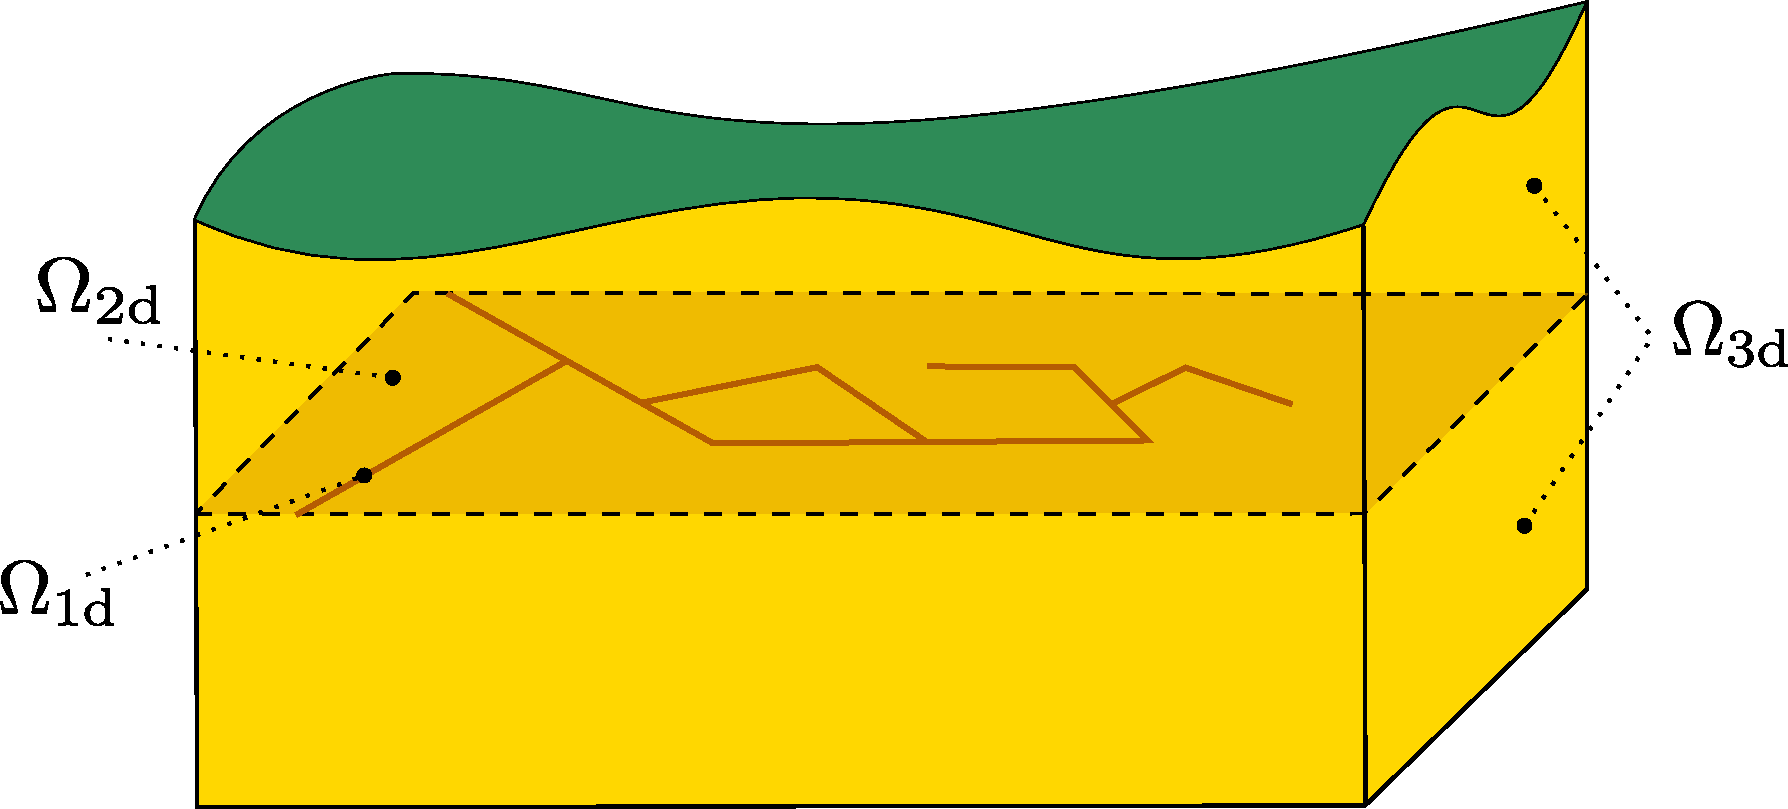
\includegraphics[width=10cm]{\fig/ground_fractures}
\caption{
    \label{fig:multi-dim}
    Scheme of a problem with domains of multiple dimensions.
}
\end{figure}

Present numerical methods used by the software require meshes satisfying the compatibility conditions
\begin{equation}
        T_{d-1}^i \cap T_d \subset \mathcal{F}_d,   \qquad \text{where } \mathcal{F}_d = \bigcup_{k} \partial T_{d}^{k}
\end{equation}
and
\begin{equation}
        T_{d-1}^i \cap \mathcal{F}_d    \text{ is either $T_{d-1}^i$ or $\emptyset$}    
\end{equation}
for every $i\in\{1,\dots, N_{E}^{d-1}\}$, $j\in\{1,\dots,N_{E}^{d}\}$,  and $d=2,3$. 
That is, the $(d-1)$-dimensional elements are either between $d$-dimensional elements and
match their sides or they poke out of $\Omega_d$. Support for a coupling between non-compatible
meshes of different dimesion is in developement and partly supported by the Darcy Flow model.


From the general point of view the problem can be seen as a strongly coupled model where the coupling is not
among physical fields but among domains of different dimensions. The coupling is then performed via boundary
conditions and source terms of the fields equations. The term 'strongly coupled' is used because the coupling 
is apparently bidirectional, the system can hardly be decoupled (meaning solving the PDEs separately). 


\section{Flow123d}
The software Flow123d is a simulator of underground water flow, solute and heat transport in fractured porous media.
It has been developed at the Technical University of Liberec approximately since 2007.
The main feature of the software is computation on on complex meshes consisting of simplicial elements of different dimensions.

Flow123d web page: \url{http://flow123d.github.io/}.


Flow123d is a simulator of underground water flow, solute and heat transport in fractured porous media. Novelty of this software is support of computations on complex meshes consisting of simplicial elements of different dimensions. Therefore, we can combine continuum models and discrete fracture network models.

Current version includes mixed-hybrid solver for steady and unsteady Darcy flow, finite volume model and discontinuous Galerkin model for solute transport of several substances and heat transfer model. Using operator splitting, we support models for various local processes including dual porosity, sorption, decays and simple reactions.

Computations can be run in parallel using MPI with scalability up to hundreds of processors. The input interface based on JSON file format allows specification of general space-time dependent data for any physical parameter that does not compromise performance. Program supports output into GMSH and VTK formats.


\section{Aim of the Thesis}
% define aims, characterize and briefly explain solution

\begin{itemize}
  \item Research of current works concerning modelling on meshes of combined dimensions, XFEM methods, Mixed-hybrid method (in particular for the Laplace equation)
        and their combination.
  \item Propose suitable enrichments for the pressure and the velocity that are stable (satisfy inf-sup condition). 
        If possible, emphasise good approximation of the velocity field which is necessary for the transport equation. 
        Enrichments to be considered: wells (point source in 2D, line in 3D), fractures (discontinuity in velocity), 
        boundary of 1D and 2D  fractures. To narrow the plan, we will concentrate on enrichment for 0D-2D and 1D-3D interaction.
  \item Implement the enrichments for 0D-2D, 1D-3D intersections in Flow123d.
\end{itemize}


%%%%%%%%%%%%%%%%%%%%%%%%%%%%%%%%%%%%%%%%%%%%%%%%%%%%%%%%%%%%%%%%%%%%%%%%%%%%%%%%%%%%%%%%%%%%%%%%%%%%%%%%%%%%%%

\chapter{State of the Art}

% current research on the problematics
% modelling on combined dimensions
% model of flow on combined dimensions
% XFEM
% theory??

%%%%%%%%%%%%%%%%%%%%%%%%%%%%%%%%%%%%%%%%%%%%%%%%%%%%%%%%%%%%%%%%%%%%%%%%%%%%%%%%%%%%%%%%%%%%%%%%%%%%%%%%%%%%%%


\section{Model of Flow on Meshes of Combined Dimensions}

In general, we are interested in the model of groundwater flow (Darcy flow considered) in fractured porous media with combined mesh dimensions.
This model can be discretised using the mixed-hybrid finite element method, which is generally described in
well known book by Brezzi and Fortin~\cite{brezzi_mixed_1991}. 
The actual application of the mixed-hybrid method in this model is studied in several articles.
In \cite{brezina_mixed-hybrid_2010}, the weak formulation and its discretization using Raviart-Thomas finite 
elements is written. The linear system is then reduced using the Schur complement (original idea in~\cite{maryska_mixed-hybrid_1995})
and solved with preconditioned conjugate gradients method.
In \cite{brezina_2012} a~mortar-like method is used to deal with discrete coupling between equations on incompatible 1D-2D meshes 
of different dimensions. The drawback of this approach is that it uses continuous approximation of velocity, so
it cannot approximate the discontinuity of the velocity over the fractures accurately enough.
In \cite{sistek_bddc_2015}, the theoretic part includes the weak and the discrete formulation and also shows
the uniqueness of the discrete solution. Further, the authors discuss application and results of BDDC 
(Balancing Domain Decomposition by Constraints) method used for solution of the linear system.

\section{eXtended Finite Element Method}

Regarding my own research, I~have been working on the following since I~started my Ph.D. study. 
I~have developed a~model for a quasi-3D aquifers-wells problem according to Gracie and Craig~\cite{gracie_modelling_2010,craig_using_2011}.
The main idea there is to use the XFEM for dealing with the singularity in pressure at the wells (0D-2D coupling).
I~have implemented different finite element methods: standard FEM with adaptive refinement, 
standard XFEM and corrected XFEM~\cite{fries_corrected_2008,fries_xfem_overview_2010},
stable generalized finite element methods (SGFEM) \cite{babuska_stable_2012, gupta_stable_2013}.
I~have measured their convergence, investigated their properties and compared them. 
I~have also improved adaptive integration on enriched elements which resulted in optimal convergence rates of
all mentioned extended finite element methods (the original integration in \cite{gracie_modelling_2010,craig_using_2011}
is not that robust and accurate enough). 
The implementation of the compared methods has been done in C++ language using the Deal II~\cite{bangerth_deal.ii_2007}, 
the finite element library not supporting any enrichment techniques at the moment.
The results are summarized in the article~\cite{exner_2016}, which is being published at the moment.

\section{XFEM on Meshes of Combined Dimensions}
There is much less to be found on the usage of XFEM in the field of flow modelling, especially regarding the dimensions coupling,
than in mechanics.
% Many researchers are using some kind of the extended finite element method, but the applications are mainly aimed
% at problems in mechanics. 
% One of the reasons is that the stability of the discrete mixed form is more sensitive 
% on the choice of the finite elements used in flow problems. 
Apart from the references on various XFEM in previous paragraph, we can name some works regarding flow and XFEM.
Extensive work has been done in the area of modelling 1D-2D fractured domains with mixed finite 
elements by D'Angelo, Fumagalli and Scotti~\cite{fumagalli_numerical_2012, dangelo_mixed_2012, fumagalli_efficient_2014}. In there, the XFEM is used to incorporate
additional degrees of freedom of zero order Raviart-Thomas basis functions on the intersected elements to allow the discontinuity
in velocity. Another work regarding 1D-2D fractures is by Schwenck~\cite{schwenck_xfem-based_2015} (also in \cite{schwenck_2015}), 
where the primary formulation is used and among others, the fracture tip and fractures intersection is dealt with.
Next, there are several publications on multi-phase fluid flow governed by Navier-Stokes equations using the XFEM for
approximation on the interfaces in 2D (\cite{diez_stable_2013,sauerland_stable_2013}). However, these are
little bit further from our application.
A 1D-3D model for investigation of the transport of substances in a~human body has been developed by D'Angelo 
and Zunino et al. (e.g in~\cite{dangelo_coupling_2008,cattaneo_numerical_2015}), without usage of XFEM.
Further, 1D-3D coupling for blood flow and mass transport in vascularized human tissue is
investigated by K{\" o}ppl in\cite{koppl_tum_2015}.


%%%%%%%%%%%%%%%%%%%%%%%%%%%%%%%%%%%%%%%%%%%%%%%%%%%%%%%%%%%%%%%%%%%%%%%%%%%%%%%%%%%%%%%%%%%%%%%%%%%%%%%%%%%%%%

\chapter{Achieved Results}
In this chapter, we shall describe the work that has already been done. First part (Section \ref{sec:model_aquifer}) 
is regarding a model of a well-aquifer system where XFEM is applied to resolve a point singularity in 2D domain. 
The second part (Section \ref{sec:elements_intersections}) is aimed at a geometrical problem of finding 
intersections of incompatible meshes of different dimensions.

\section{Model of Well-Aquifer System} 
\label{sec:model_aquifer}
The content is based on our publication \cite{exner_2016}. Some problems with convergence addressed in the article
have been solved since its accepting, the test problem has been modified and also an alternative integration technique
using polar coordinates has been suggested.

\subsection{Model equations}
We consider a steady groundwater 
flow in a system of aquifers (2D models of horizontal geological layers) separated by aquitards. 
In contrast to Gracie and Craig \cite{gracie_modelling_2010}, we suppose the aquitards to be impermeable, 
however we add an artificial volume source term. This allows us to better study the impact of 
the prescribed source on the solution which is better suited to the numerical experiments we are focused on. 

The aquifers are then connected only through the wells 
which act as sources or sinks in the domain of each aquifer. The pressure in the aquifers is further governed 
by a Dirichlet boundary condition on the outer boundary of every aquifer.

The model is defined as a complex multi-aquifer system to follow our implementation and to see the differences
we made in comparison to Gracie and Craig. Although later, we consider mostly just single aquifer.

Let $\Theta^m\subset \Real^2$ be the domain of the $m$-th aquifer, $m=1,\ldots M$.
The well $w\in\mathcal{W}=\{1,\ldots,W\}$ is represented by an infinite vertical cylinder $B_w$
with center $\bx_w$ and radius $\rho_w$.  We further denote 
\[
 B^m_w = B_w \cap \Theta^m, \quad \text{and} \quad
 B^m=\bigcup_{w\in \mathcal{W}}B^m_w,
\]
for any aquifer $m$ and a well $w$.
The actual computational domain of the aquifer $m$ is $\Omega^m = \Theta^m\setminus B^m$. The boundary $\partial\Omega^m$ of 
the domain consists of the exterior part $\partial\Theta^m=\Gamma^m_D$ and the interior part $\partial B^m$.


Combining the Darcy law and the continuity equation for incompressible fluid, we get
a Poisson equation for the pressure head in the $m$-th aquifer:
\begin{equation} \label{eqn:poisson}
\nabla\cdot(-\mathbf{T}^m\nabla h^m) = f^m \qquad \textrm{on } \Omega^m\subset\Real^2,\; \forall m=1,\dots,M, \\
\end{equation}
which has to be supplied with boundary conditions
\begin{align}
h^m|_{\Gamma^m_D} &= h^m_D, \\
\label{eq:interior_bc}
\left(-\mathbf{T}^m\nabla h^m\cdot\vc{n}\right)|_{\partial B^m_w} &= \sigma^m_w(\langle h^m \rangle - H^m_w) \qquad \forall w\in\mathcal{W},
\end{align}
%
% \noteJB{Na vrtu by mel byt predepsany konstantni tok dany prumerem tlaku, tj.pomoci $Q_w^m$. 
% Pak se nam objevi prumery i v nekterych dalsich rovnicich. Jde, jde o to s jakou implementaci to bylo pocitane. To bych tam nechal bez ohledu na to ze
% spravne je nektera z moznych formulaci s prumerama.
% }
where $\mathbf{T}^m\, [\textrm{m}^2\textrm{s}^{-1}]$ denotes the transmissivity tensor,
%(we will further consider only scalar $T^m$ for simplicity), 
$h^m\, [\textrm{m}]$ is the pressure head, $f^m\, [\textrm{m}\textrm{s}^{-1}]$ stands for the source density,
$\vc{n}$ is the unit outer normal vector of the interior boundary (i.e. pointing to the centers of wells),
$\sigma^m_w\, [\textrm{m}\textrm{s}^{-1}]$ denotes the permeability coefficient between $w$-th well and 
$m$-th aquifer, and finally $H_w^m$ is the pressure head in the well $w$ at the level of $m$-th aquifer.
%
\begin{figure}[!htb]
  %\vspace{-15pt}
  \begin{center}         
    \def\svgwidth{0.5\textwidth}
    \input{\figpath well_communcation.pdf_tex}
  \end{center}
  \caption{Flow balance in the well.}
  \label{fig:well_flows}
\end{figure}
%
The average value of pressure head along the well edge $\langle{h^m}\rangle$ is defined as
\[\langle{h^m}\rangle = \fint_{\partial B_w} h^m  \dd\bx.\]
The boundary condition with the average pressure head $\langle{h^m}\rangle$ forces the gradient
of the pressure head to constant.

The total flow from the well $w$ to aquitard $m$,
\[
    Q^m_w =-\int_{\prtl B^m_w} \sigma^m_w(\langle h^m \rangle - H^m_w)  \dd\bx
\]
satisfies a simple balance equation on the well
\begin{align}
    \label{eq:well_flow}
    Q_w^m = Q^m_{w,in} - Q^m_{w,out} = c^{m+1}_w\left( H^{m+1}_w-H^m_w \right) - c_w^m\left( H^m_w-H_w^{m-1}\right),&\\
    \notag
    \forall\,m=1,\dots,M\text{ and }\forall\,w\in\mathcal{W},&
\end{align}
where $Q^m_{w,in}$ is the flow from the upper aquifer $m+1$, $Q^m_{w,out}$ is the flow to the lower aquifer $m-1$, and 
$c^m_w\, [\textrm{m}^2\textrm{s}^{-1}]$ is the permeability of the well $w$ in the segment below the aquifer $m$.

%
In \eqref{eq:well_flow}, we assume Darcy flow in the well for the simplicity. The bottom of the well $w$ is impermeable,
we set $c^1_w=0$, $H^0_w=H^1_w$ there, and we prescribe given pressure $H^{M+1}_w$ at the top.

%refer to the article

\subsection{Weak formulation}
We define the trial space $V$ and the test space $V_0$:
\begin{eqnarray} \label{eqn:spaces}
  V &=& \left(H^1(\Omega^m)\right)^M\times\Real^{W(M+1)}, \\
  V_0 &=& \left(H^1_0(\Omega^m)\right)^M\times\Real^{WM},
\end{eqnarray}
where $H^1(\Omega^m)$ is the standard Sobolev space and 
\[ H^1_0(\Omega^m)=\{\varphi\in H^1(\Omega^m); \varphi|_{\Gamma^m_D}=0\}. \]
We can now introduce the weak solution $u$ and the test function $v$
\begin{eqnarray} \label{eqn:solution}
   u &=& (h^1,\ldots, h^M, H^1_1,\ldots,H^{M+1}_W)\in V, \\
   v &=& (\varphi^1,\ldots, \varphi^M, \Phi^1_1,\ldots,\Phi^M_W)\in V_0.
\end{eqnarray}
We understand $V_0$ as a subspace of $V$ setting $\Phi^{M+1}_W=0$.

To obtain the weak form, we apply the standard Galerkin method. We multiply the equation \eqref{eqn:poisson} 
by a test function $\varphi^m$ and integrate by parts over $\Omega^m$, for all $m=1,\ldots,M$, to get
\begin{equation} \label{eqn:weak_form1}
  \int_{\Omega^m} T^m \nabla h^m \cdot \nabla \varphi^m \dd\bx
  + \sum_{w\in \mathcal{W}} \int_{\partial B^m_w} \sigma^m_w (\langle h^m \rangle - H_w^m) \varphi^m \dd\bx
  = \int_{\Omega^m} f^m\varphi^m \dd\bx.
  % - \int \limits_{\Omega^m} T^m \nabla h^m_D \nabla v^m \dd\mathbf{x},
\end{equation}
%
We then multiply \eqref{eq:well_flow} by $\Phi^m_w$, add it to \eqref{eqn:weak_form1} 
and sum up over $m$ which results in
\begin{multline} \label{eqn:weak_form}
  \sum_{m=1}^M \; \int_{\Omega^m} T^m \nabla h^m \cdot \nabla \varphi^m \dd\bx
        + \sum_{m=1}^M \sum_{w\in \mathcal{W}} \; 
           \int_{\partial B^m_w} \sigma^m_w\left(\langle h^m \rangle-H^m_w\right)\left(\langle \varphi^m \rangle -\Phi^m_w\right) \dd\bx \\
        + \sum_{m=1}^{M+1} \sum_{w\in\mathcal{W}}
          c_w^{m}\left( H^{m}_w-H_w^{m-1}\right)\left(\Phi^{m}_w - \Phi^{m-1}_w\right)           
  = \sum_{m=1}^M \; \int_{\Omega^m} f^m\varphi^m \dd\bx.   
\end{multline}
% \noteJB{Consider sum over aquifers to get square term from communication on wells.
% Boundary conditions on wells?}
We say that $u\in V$ is a weak solution if it satisfies \eqref{eqn:weak_form} for all $v\in V_0$. 
Putting $h^m=\varphi^m$ and $H^m_w=\Phi^m_w$, we can clearly see the elliptic character of all terms on the 
left hand side of the weak form \eqref{eqn:weak_form} in the whole test space $V_0$. The existence and uniqueness of the solution can be shown 
via the Lax-Milgram lemma due to ellipticity and boundedness of the problem.

\subsection{Discretization}
\label{sec:discretization}
We can now proceed to the choice of the enrichment and discretization of the equation \eqref{eqn:weak_form}.
In this section as well as in the rest of the paper, we shall consider only one aquifer for the sake of simplicity
so we can omit the upper index $m$. Extension to the multi-aquifer system is straightforward. 
In particular, the space of shape functions is same on every aquifer since we consider 
the same triangulation for every aquifer in our implementation. 
Namely, we use regular square grid.

\subsubsection{Enrichment function}
The enrichment function can be obtained from the solution of a local problem on the neighborhood of the well $w$.
Let $\Omega_w$ be an annulus with center $\vc x_w$ inner radius $\rho_w$ and arbitrary outer radius $D \gg \rho$.
Solution of the Laplace equation $-T \Delta h = 0$ on $\Omega_w$ with any radially symmetric boundary conditions has a form
%
\begin{equation} \label{eqn:solution_form}
  h = a \log(r_w)+b, %\quad \textrm{where }
\end{equation}
where $r_w$ is a distance function
\begin{equation} \label{eqn:distance}
r_w(\bx) = \|\\bx - \bx_w\|= \sqrt{(x-x_w)^2+(y-y_w)^2}.
\end{equation}
%
Thus the pressure head would go to infinity while closing to the center of the well.
Keeping in mind the radius of the well $\rho_w$ and the local solution \eqref{eqn:solution_form}, 
we introduce a (global) enrichment function
%
\begin{equation}
\label{eqn:enrich_func}
s_w(\bx) = 
  \begin{cases}
  \log(r_w(\bx)) & r_w > \rho_w,\\
  \log(\rho_w) & r_w \le \rho_w.\\
  \end{cases}
\end{equation}
See \fig{fig:enrich_func}.
It is natural to use the same $s_w$ on each aquifer since it depends only on $r_w$ and the wells have constant center and radius along the $x$-axis
(we consider only vertical wells, perpendicular to aquifers).
%
% and its gradient
% \begin{equation} \label{eqn:xgrad_func}
% \nabla s_w(\bx) = 
%   \begin{cases}  
%     \frac{\bx - \bx_w}{r_w^2(\bx)} & r_w>R_w \\
%     0 & r_w \leq R_w
%   \end{cases}.
% \end{equation}

%\notePE{DONE: do not forget to replace the notation of the enrichment function}
\begin{figure}[!htb]
  %\vspace{-15pt}
  %TODO: do not forget to replace the notation of the enrichment function
  \begin{center}         
    \def\svgwidth{0.5\textwidth}
    \input{\figpath enrich_func.pdf_tex}
  \end{center}
  \caption{The enrichment function.}
  \label{fig:enrich_func}
\end{figure}


In contrast to global enrichment methods, the XFEM and the SGFEM apply the enrichment functions only locally. 
Since the enrichment function is radial, it is natural to consider the enriched domain $Z_w = B_{R_w}(\vc x_w)$
of the well $w$ given by the enrichment radius $R_w$. Local enrichment methods enrich only 
nodes that are in the enriched domain of at least one well.

\subsubsection{Partition of unity methods}
\label{sec:pum_methods}
Let $N_\alpha(\bx)$, $\alpha\in\mathcal{I}=\{1,\ldots,N\}$ be the standard linear finite element shape 
functions associated with the node $\bx_\alpha$ of the triangulation. 
In the \textbf{standard XFEM}, we write the solution in the form
\begin{equation} \label{eqn:xfem_standard_form}
  h(\bx) = \sum_{\alpha\in\mathcal{I}}a_\alpha N_\alpha(\bx)
    + \sum_{w\in\mathcal{W}} \sum_{\alpha\in\mathcal{I}^e_w} b_{\alpha w} \phi_{\alpha w}(\bx),
\end{equation}
where $a_\alpha$ are the standard FE degrees of freedom and $b_{\alpha w}$ are the degrees of freedom coming from
the enrichment of the well $w$. The index set $\mathcal{I}^e_w$ includes all nodes enriched by the well $w$; on the other hand, 
at one node one can have several enrichment functions originating from different wells.
The local enrichment functions $\phi_{\alpha w}$ in \eqref{eqn:xfem_standard_form} are defined
in the following way
\begin{equation} \label{eqn:xfem_enrich}
    \phi_{\alpha w} = N_\alpha(\bx)L_{\alpha w}(\bx), \quad \alpha\in\mathcal{I}^e_w, w\in\mathcal{W},
\end{equation}
where the enrichment function is simply $L_{\alpha w}(\bx) = s_w(\bx)$.

\subsubsection{Corrected XFEM}
The corrected XFEM, introduced in  \cite{fries_corrected_2008}, deals with the convergence problem on blending elements
which are elements on the boundary of the enriched zone that contains both enriched and unenriched nodes.
The corrected XFEM introduces the \textbf{ramp function}
\begin{eqnarray} \label{eqn:ramp_function}
  G_w(\bx) &=& \sum_{\alpha\in\mathcal{I}_w^e} N_\alpha(\bx)    \\
  &=& 
  \begin{cases}
    0 & \textrm{ on unenriched elements,}    \\
    1 & \textrm{ on elements where all nodes are enriched,}    \\
    ramp & \textrm{ on elements where some of the nodes are enriched.}    \\
  \end{cases} \nonumber
\end{eqnarray}
It also extends the set of the enriched nodes of the well $w$, denoted by $\mathcal{J}^e_w$, by enriching also (previously unenriched) nodes 
of the blending elements of the well $w$. Thus $\mathcal{I}^e_w\subset\mathcal{J}^e_w$.
The enrichment function changes into the form
\begin{equation} \label{eqn:xfem_ramp}
    L_{\alpha w} = G_w(\bx) s_{w}(\bx), \quad \alpha\in\mathcal{J}^e, w\in\mathcal{W}.
\end{equation}


In the same work, i.e. \cite{fries_corrected_2008}, authors further suggest the \textbf{shifted} enrichment functions in order 
to preserve the property of the standard 
FE approximation at nodes $h(\bx_\alpha)=a_\alpha$: the value at the node is equal to the corresponding degree
of freedom. The enrichment functions must be then zero at the nodes which is satisfied in the form
\begin{equation} \label{eqn:xfem_shift}
    L_{\alpha w} = G_w(\bx) \left[s_w(\bx) - s_w(\bx_\alpha)\right],
    \quad \alpha\in\mathcal{J}^e, w\in\mathcal{W}.
\end{equation} 
The property of the shifted formulation enables us to prescribe Dirichlet boundary condition such that
$a_\alpha = h_D(\bx_\alpha)$.

It has been also shown in many cases that both ramp function and shifting are needed to obtain optimal convergence rate.
In \cite{ventura_fast_2009}, authors analyse a more general form of a ramp function (calling the method a weighted XFEM)
and compare different alternatives of shifting on crack and dislocation problems. The methods described above can be then seen
as special types of the weighted XFEM. Let us call them the \textbf{ramp function XFEM}  
and the \textbf{shifted XFEM} for the purpose of this article, as we shall reference to them later.

\subsubsection{SGFEM}
Finally, we present the \textbf{SGFEM}, according to \cite{babuska_stable_2012,gupta_stable_2013}. 
The enrichment function is defined as the subtraction of the global enrichment function and its interpolation 
\begin{equation} \label{eqn:sgfem_enrich}
    L_{\alpha w}|_{\tau} = \left[s_w(\bx) - \pi_\tau (s_w)(\bx)\right],
    \quad \alpha\in\mathcal{I}^e_w, w\in\mathcal{W}.
\end{equation} 
for any element $\tau$ of the mesh that have at least one enriched node.
The interpolation $\pi_\tau$ is built using the finite element shape functions
associated with nodes $\mathcal{I}(\tau)$ of the element $\tau$
\begin{equation} \label{eqn:sgfem_interpolation}
    \pi_\tau (s_w)(\bx) = \sum_{\beta\in\mathcal{I}(\tau)} s_w(\bx_\beta) N_\beta(\bx).
    %\quad \textrm{ on } \tau,\; \alpha\in\mathcal{I}^e, w\in\mathcal{W}.
\end{equation}
Notice that there are no additional enriched nodes on blending elements, like in $\mathcal{J}^e$ in 
\eqref{eqn:xfem_ramp} and \eqref{eqn:xfem_shift}, and no ramp function is involved.


\subsection{Integration on enriched elements}
\label{sec:integration}
In order to compute the entries of the system matrix, %\eqref{eqn:s_entry} and \eqref{eqn:r_entry} 
we need to integrate
the expressions containing the enrichment functions. These of course can be non-polynomial, like they are 
in our case. The standard quadrature rules are not appropriate any more, for they are constructed to integrate 
precisely only polynomials up to a given degree. The higher requirements on the integration precision
are the price for using enrichment functions and a coarse mesh.

There are two aspects which the integration must handle properly:
\begin{itemize}
  \item the steep gradient of enrichment base functions in the vicinity of the well (the singularity),
  \item the well edge geometry, since we need to integrate only outside of the well.
\end{itemize}

One of the approaches to deal with these requirements is an adaptive quadrature. The element is divided into 
subregions (squares on the reference element) only to place more quadrature points inside but not to bring 
any more degrees of freedom into the system. In this section we will discuss the adaptivity rules, 
suggest an improvement and compare our strategy to the original one (developed in \cite{gracie_modelling_2010}).

\subsubsection{Instability of adaptive quadrature}
\label{sec:refinement_element}
Gracie and Craig in \cite{gracie_modelling_2010} refine only subregions that cross the boundary of the well, using at most 12 refinements.
This catches nicely the well edge but it works only when the well is placed at the node of an element or near the center of an element. 
When the well is placed near the edge of an element, there can be
a large difference in the size of neighboring subregions, see \fig{fig:adapt_ref_a}. Although
the integrand is computed precisely enough on the element with the well inside, the quadrature points on the
neighboring elements (where the integrand has still large derivatives) are placed very sparsely 
and the integration error is large.

\begin{figure}[!htb]
%   \vspace{0pt}
  \centering    
  \subfloat[refinement due to Gracie and Craig]{\label{fig:adapt_ref_a} 
    \includegraphics[width=0.45\textwidth]{\figpath adaptive_refinement_3_old.pdf} }
  \hspace{0pt}
  \subfloat[improved refinement]{\label{fig:adapt_ref_b} 
    \includegraphics[width=0.45\textwidth]{\figpath adaptive_refinement_3_new.pdf} }
  \caption[Adaptive refinement comparison]
  {Comparison of the original and improved refinement techniques.
   Black lines denote enriched elements edges, red lines denote adaptive refinement (subregions edges) and the well
   edge is blue.
  }
  \label{fig:adapt_refinement}
\end{figure}
In order to overcome this instability of the adaptive quadrature, we have made an asymptotic analysis of the integration error presented 
in the next section.

\subsubsection{Estimate of quadrature error}

Let us assume only one well of radius $\rho$ situated at the origin. In the case of elliptic equation, the term with the strongest singularity is 
\begin{equation}
    \label{eq:term-of-interest}
    f(r)=(\nabla \log r )^2 \approx r^{-2}
\end{equation}
which is also the worst term to integrate independently of the particular variant of the PU method.
Consider a~square subregion $S$ with a~side $\delta$ and 
let us denote $r_{S}$ its distance from the origin.
We want to estimate the error of the 2D tensor product Gauss quadrature rule of order $n$ ($n$ times $n$ points) on the square $S$. 
Let us denote 
$\Pi^n f$ the projection of the integrand $f$ to the space of polynomials that are integrated exactly.
We were not able to find error estimates for 2D quadratures in the literature and deriving them would be extremely technical.
However, we can make an observation that among the squares of the same $r_{S}$, the quadrature error is the highest for the squares laying on one of the axis.
Assume without loose of generality a square on the $X$-axis. Since $\abs{y}<\delta \ll \abs{x}$, the monomials of $\Pi^n f$ containing $y$ 
are negligible and we get the quadrature
of order $n$ in the radial ($X$-axis) direction. On the other hand for the square on the diagonal, the bilinear terms of 
a 2D quadrature effectively enhance its order to $2n$ in the radial (diagonal) direction. Due to the radial nature of the integrand,
we can estimate the quadrature error on the square $S$ by the error on the square $S'$ with the same $r_S$ laying on the $X$-axis, then we can 
neglect $y$~monomials and use the error estimates for the 1D quadrature:
\[
  \int_S \abs{f-\Pi^n f} \dd\bx \le \int_{S'}\abs{f-\Pi^n f} \dd\bx \le \delta E^n((r_{S}, r_{S}+\delta)).
\]
The $E_n$ is the error of 1D Gauss quadrature of the order $n$ ($n$ quadrature points) over the interval $(r,r+\delta)$
\[
  E_n = \frac{\delta^{2n+1} (n!)^4}{(2n+1)((2n)!)^3} f^{(2n)}(\xi_n) 
\]
for some $\xi_n \in (r, r+\delta)$, see e.g. \cite{kahaner_numerical_1989}. 
The expression $f^{(2n)}$ denotes a derivative of order $2n$ of a function $f$.
Regarding the integrand \eqref{eq:term-of-interest}, we have 
\[
  \abs{f^{(2n)}(r)} = (2n+1)! r^{-(2n+2)}.
\]
Finally, we get an estimate for the quadrature error on a single subregion:
\[
    \int_S \abs{f-\Pi^n f}  \dd\bx \le  \alpha_n \left( \frac{\delta}{r_{S}} \right)^{2n+2}, 
  \qquad \alpha_n = \left( \frac{(n!)^2}{(2n)!} \right)^2.
\]
This estimate implies that we have to ensure $\delta < r_S$ in order to get a decent quadrature error 
and possibly to employ a higher order quadrature. 


%JB%Derived criterion holds only on squares, where the integrated function is smooth.
%JB%This is not the case for squares intersecting the boundary of the well, $r_{S} \le \rho \le r_{max}$, where we integrate 
%JB%discontinuous function $\chi_{S \setminus W} f$. Using substitution, we can map $W$ to unit circle $B$
%JB%\[
%JB%  \int_{S} \chi_{S \setminus W} \frac{1}{r^2} \d \vc r= \int_{S'} \chi_{S' \setminus B} \frac{1}{r'^2} \d \vc {r'},
%JB%\]
%JB%where $S'$ is square with side $H=\delta/\rho$ and $\vc {r'} = \vc{r}/\rho$. Empirically determined error of the midpoint rule for later 
%JB%integral is
%JB%\[
%JB%    E(H) = c_e H^{p_e}, \quad \text{with } c_e=0.08,\ p_e=2.5.
%JB%\]
%JB%This error has to be smaller then $\epsilon h^2$, thus for $h$ we get formula:
%JB%\begin{equation} \label{eqn:h_criterion}
%JB%   h\le h_b(\epsilon) = \Big(\frac{\epsilon \rho^{p_e}}{c_e}\Big)^{\frac{1}{p_e-2}}. 
%JB%\end{equation}
%JB%
%\noteJB{TODO: modify test of integration on unit disk for the function $1/r^2$.}

\subsubsection{A priori adaptive quadrature rules}
Let us denote $r_{min}$ the minimum and $r_{max}$ the maximum distance to the center of a well from a subregion. 
Based on the analysis presented above, we propose following adaptive quadrature rules:
%JB%\begin{enumerate}
%JB% \item If $r_{max} < \rho$ the square quadrature is zero.
%JB% \item If $r_{min} < \rho < r_{max}$ (square cross the well boundary) we subdivide the square unless $\delta < 2^{-12}h$.
%JB% \item If $r_{min} > \rho$. For $\frac{h}{r_{min}} > \frac{1}{2}$ subdivide the square, else select order $n$ so that 
%JB% \begin{equation} \label{eqn:alpha_criterion}
%JB%    \frac{\alpha_n h^{2n}}{r_{min}^{2n+2}} \le \epsilon,
%JB% \end{equation}
%JB% use at least the same order as necessary for FEM.
%JB%\end{enumerate}
%JB%
%\noteJB{TODO:
%We should estimate true error numerically using one more subdivision and compare it to prescribed tolerance, we should be safely 
%below, without increasing the number of evaluation compared to current implementation.
%}



%JB%We suggest additional criterion for subelements refinement which takes into account a subelement diameter 
%JB%and its distance from the well
%JB%\begin{equation}
%JB%  h \leq C_R r_{min},
%JB%\end{equation}
%JB%\notePE{Originally, I compute $r_{min}$ between vertices and the well center, but I believe that the results would be the same.}
%JB%where $h$ is the diameter of the subelement and $r_{min}$ is the minimal distance between a vertex of 
%JB%the subelement and the well center. $C_R$ is a scaling constant, equal 0.5 by default, through which we can 
%JB%control the significance of the criterion. If satisfied, the subelement is not refined anymore.
%JB%

%JB%Eventually, we do 10 levels of improved adaptive refinement with the following rules ($r_{max}$ is the maximal
%JB%distance of a vertex of the subelement and the well center):
\begin{enumerate}
 \item If $r_{max} < \rho$, the subregion is not refined and the quadrature is zero.
 \item If $r_{min} < \rho < r_{max}$ and $\delta > 2^{-10}h$, the subregion is refined.
 \item If $r_{min} < \rho < r_{max}$ and $\delta \le 2^{-10}h$, $3\times3$ Gauss quadrature is used.
 The values at quadrature points lying inside the well are set to zero.
 \item If $r_{min} > \rho$ and $\delta > r_{min} / 2$, the subregion is refined.
 \item If $r_{min} > \rho$ and $\delta \le r_{min} / 2$, $3\times3$ Gauss quadrature is used.
\end{enumerate}


These rules ensure $\delta < r_{min}/2$ outside the well, where the integrand is smooth. Subregions intersecting 
the well's boundary are refined using at most $10$ refinement levels, since the integrand is discontinuous there and we cannot employ 
estimates from the previous section. The maximum number of levels is chosen so that we get the similar total number of quadrature points 
as in the quadrature used by Gracie and Craig in \cite{gracie_modelling_2010}. Using the proposed rules, the elements that do not contain the well are refined as well,
see \fig{fig:adapt_ref_b}. 

Implementation of this approach allows the convergence rates of the used PU methods to close up to the optimum,
as the results of the numerical tests will show in section \ref{sec:results}.

\subsubsection{Quadrature in polar coordinates}

The idea for the usage of the quadrature in polar coordinates originates from the radial character of the terms
that are integrated. 
The motivation is to reduce the number of quadrature points (refinement levels) of the previously described quadrature due to
precise representation of the well edge.

We define a circular neighbourhood of a well, i.e. a band of width $\gamma$ (see \fig{fig:well_band}),
\[ \mathcal{P} = \{\vc{x}: \rho < \abs{\vc{x} - \vc{x}_w} < \rho + \gamma \}.\]
Next we define a smooth step function (see \fig{fig:smooth_step})
\[\mu(z) = -2 z^3 +3 z^2,\quad z=\frac{r-\rho}{\gamma}.\]%
%
\begin{figure}[!htb]
  \vspace{-35pt}
  \centering    
  \subfloat[refinement due to Gracie and Craig]{\label{fig:well_band} 
          \def\svgwidth{0.35\textwidth}
          \input{\figpath well_band.pdf_tex}
  }
  \hspace{0pt}
  \subfloat[improved refinement]{\label{fig:smooth_step} 
          \def\svgwidth{0.5\textwidth}
          \input{\figpath smooth_step.pdf_tex}
  }
  \caption[Smooth step function]
  {Smooth step function $\mu$ on the well neighbourhood $\mathcal{P}$.
  }
  \label{fig:smooth_step_well_band}
\end{figure}    

We use $\mu$ as a partition of unity to divide an integral into 2 parts
\begin{eqnarray} 
      \int\limits_S v(\mathbf{x}) \dd \mathbf{x} &=& \int\limits_S \mu(r) v(\mathbf{x}) \dd \mathbf{x} + \int\limits_S (1-\mu(r)) v(\mathbf{x}) \dd \mathbf{x} \nonumber\\
      &=& \int\limits_S \mu(r) v(\mathbf{x}) \dd \mathbf{x} + \int\limits_0^{2\pi} \int\limits_\rho^{\rho+\gamma} (1-\mu(r)) v(\mathbf{x}) r \dd r \dd \phi.
\end{eqnarray}
We see that the first integral vanishes when closing to the well edge, while the second grows. This corresponds
to the character of the solution which is more radial in the vicinity of the well rather than far away from it.
Therefore we transform the second integral into polar coordinates $\mathbf{x} \longleftrightarrow (r,\phi)$. 
The first integral is computed using the previously described quadrature, but with much less refinement
levels, since the well edge is now represented precisely (see \fig{fig:polar_quad_points} with
an example of quadrature points distribution).
%
\begin{figure}[!htb]
%   \vspace{0pt}
  \centering    
  \subfloat[$\int\limits_\Omega \mu(r) v(\mathbf{x}) \dd \mathbf{x}$]{\label{fig:adapt_ref_polar_a} 
         \includegraphics[width=0.47\textwidth]{\figpath adaptive_refinement_well.pdf}
  }
  \hspace{0pt}
  \subfloat[$\int\limits_0^{2\pi} \int\limits_\rho^{\rho+\gamma} (1-\mu(r)) v(\mathbf{x}) r \dd r \dd \phi $]{\label{fig:adapt_ref_polar_b} 
          \includegraphics[width=0.47\textwidth]{\figpath polar_band_refinement.pdf}
  }
  \caption[Polar quadrature points]
  {Distribution of quadrature points of the two integral parts.
  }
  \label{fig:polar_quad_points}
\end{figure} 

The adaptive integration in polar coordinates has been implemented and tested.
However, the results of are not satisfying as expected. The quadrature accuracy is very dependent on the choice of
the band with around the well, position of the well relative to nodes of the mesh and also to the size of nearby elements.
When playing long enough with the setting, an optimal convergence rate can be reached, but no general and robust 
setting has been found. The problematics would need a deeper investigation and we leave it open for now, since
we can still use the previously described quadrature.


%JB%\subsection{Adaptive integration experiment}
%JB%We now describe the experiment from which we obtained the coefficients in the criterion 
%JB%\eqref{eqn:h_criterion}. Let us have a single element, a square $4\times4$, out of which a circle of unit radius 
%JB%is cut off -- this represents an element with a well. We now want to investigate integration error
%JB%in the vicinity of the circle on the function $f=r^{-2}$, $r$ being the distance from the center of the circle. 
%JB%
%JB%We compute the integral on the selected level of refinement only on the squares intersecting the circle. Then
%JB%we refine the squares up to the 12-th level, integrate again and compute the difference. Quadratures rules
%JB%$1\times1$, $2\times2$, $3\times3$ and $4\times4$ are used. The results are shown in 
%JB%\fig{fig:adapt_integration_conv} also with convergence trend lines equations. The conclusion can be made
%JB%that it is more efficient to refine one more level with one-point quadrature than to use higher order 
%JB%quadrature on the coarser level. As for the coefficient, these can be read from the graph -- for the one point
%JB%quadrature $c_e=12.65$ and $p_e=1.27$.
%JB%
%JB%\begin{figure}[!htb]
%JB%%   \vspace{0pt}
%JB%  \centering    
%JB%  \includegraphics[width=0.9\textwidth]{results/adapt_integration_conv.pdf}
%JB%%   \subfloat[rozdìlený element s vrtem]{\label{fig:adapt_ref_a} 
%JB%%     \includegraphics[width=70mm]{\figpath adaptive_ref.pdf} }
%JB%%   \hspace{0pt}
%JB%%   \subfloat[detail hranice vrtu]{\label{fig:adapt_ref_b} 
%JB%%     \includegraphics[width=72mm]{\figpath adaptive_ref_detail.pdf} }
%JB%  \caption[Adaptive quadrature convergence.]{Convergence graph of adaptive quadrature on function $r^{-2}$.
%JB%  \\ \notePE{thicker trend lines}}
%JB%  \label{fig:adapt_integration_conv}
%JB%\end{figure}
%JB%
\subsection{Estimate of the enrichment radius} \label{sec:enrichemnt_radius}
In this section, we shall study the dependence of the solution error on the enrichment radius $R$. First part is devoted to 
theoretical analysis, the later part presents numerical results.
Let us consider a general elliptic problem to find $u\in V$ satisfying
\[
   a(u, \phi) = \langle f, \phi \rangle, \text{ for } \phi \in V,
\]
where $a$ is bounded elliptic bilinear form: $\norm{a}\le M_a$, $a(v, v) \ge \gamma \norm{v}_V^2$, $\gamma>0$, and $f$ a bounded linear form, $f\in V'$. 
Suppose, that the problem is to be solved on a domain $\Omega \subset \Real^2$ with a single hole (well) of radius $\rho$ at the origin. 
Let us assume, that the solution can be split into the singular part $u_s(\vc x)= \log |\vc x|$ and the regular part $u_r=u-u_s$.
Let $V^P_h$ be a polynomial finite element subspace of $V$ on a regular mesh of elements with a maximal diameter $h$
and let $V_h$ be a such enriched space that $u_s$ can be approximated exactly on the enriched domain $Z_R$, i.e.
\[
   \inf_{v\in V_h} \norm{u_s - v}_V = \inf_{v\in V^P_h} \norm{u_s|_{Z'_R} - v}_V, \quad Z'_R = \Omega\setminus Z_R.
\]
Using standard error estimate for elliptic PDE (e.g. \cite[Theorem 13.1]{ciarlet_basic_1991}), we get
\begin{equation}
    \label{eq:std_err_estimate}
    \norm{u - u_h}_{V} \le c_a \inf_{v \in V_h} \norm{u - v}_{V} 
    \le c_a \big(\inf_{v \in V^P_h} \norm{u_r - v}_{V} + \inf_{v \in V_h} \norm{u_s - v}_{V} \big).   
\end{equation}
where $c_a=1+\norm{a}/\gamma$.
In the following, we consider $V=H^1(\Omega)$, square grid and $V^P_h$ formed by bilinear finite elements. 
Then \eqref{eq:std_err_estimate} can be further estimated using approximation property of $V^P_h$:
\begin{equation}
    \label{eq:particular_estimate}
    \norm{u - u_h}_{H^1(\Omega)} \le c_a \big(c h \abs{u_r}_{H^2(\Omega)} + \norm{u_s - \Pi u_s}_{H^1(Z'_R)} \big)   
\end{equation}
where $\Pi u_s$ denotes interpolation of $u_s$ in $V^P_h$. Our next aim is to find tight estimate for the second term.
To this end, we calculate $H^1$ error on a single square element $S_{h,r}$ with side $h$ and distance $r$ from origin.
Using parametrization $0<s,t<1$,  we get

\begin{align*}
 (u_s - \Pi u_s)(s,t)&=\log\sqrt{(r+hs)^2+(ht)^2} -\Big[(1-s)(1-t)\log r\\
 &\quad+ (1-s)t\log\sqrt{r^2+h^2} + s(1-t) \log(r+h) \\
 &\quad+ st\log\sqrt{(r+h)^2+h^2} \Big]\\
 &=\frac12 \frac{h^2}{r^2}\big(t^2-t - s^2 +s\big) + O(\frac{h^3}{r^3})
\end{align*}
and 
\begin{equation}
 \nabla(u_s - \Pi u_s)(s,t) = \frac{h}{r^2} \Big( \frac12-s, t-\frac12 \Big) + O(\frac{h^2}{r^2}).
\end{equation}
Assuming $h<r$, we can neglect higher order terms. Then, we obtain by direct integration
\begin{align*}
 \norm{u_s - \Pi u_s}^2_{L^2(S_{h,r})} \approx \frac14 \frac{h^6}{r^4}\int_0^1\int_0^1 (t^2-t-s^2+s)^2\,\dd s\, \dd t = \frac{1}{360}\frac{h^6}{r^4} 
\end{align*}
and
\begin{equation}
    \label{eq:grad_estimate_on_square}
    \norm{\nabla(u_s - \Pi u_s)}^2_{L^2(S_{h,r})} \approx \frac{2h^4}{r^4} \int_0^1 \Big(t-\frac12\Big)^2 \dd t = \frac{1}{6}\frac{h^4}{r^4}.
\end{equation}
Thus for the density of squared error we have
\[
    \frac{1}{\abs{S_{h,r}}} \norm{u_s - \Pi u_s}^2_{H^1(S_{h,r})} \approx \frac{h^2}{6r^4}
\]
which after integration over the unenriched domain gives final estimate:
\begin{equation}
    \label{eq:singular_approx_error}
    \norm{u_s - \Pi u_s}_{H^1(Z'_R)} \le \left[\int_0^{2\pi} \int_R^\infty \frac{h^2} {6r^4} r \,\dd r\, \dd \phi\right]^{1/2} = \sqrt\frac{\pi}{6}\frac{h}{R}. 
\end{equation}

Recalling the estimate \eqref{eq:std_err_estimate}, we can conclude that optimal choice of the enrichment radius is $h/R\approx \norm{u_r-\Pi u_r}_{H^1(\Omega)}$, 
which balance error in the regular and the singular part. In combination with an a posteriori error analysis, this could give a rule for an automatic
determination of the enrichment radius.



\subsection{Numerical results}
\label{sec:results}

\subsubsection{Test problems} \label{sec:test_cases}
In this section, we define problems that we solve in our numerical experiments. We restrict ourselves to 
single aquifer problems for the purpose of this article but our implementation enables multi-aquifer systems 
as well. In order to measure convergence, it is desirable to have an analytic solution which will be also derived. 

Consider the following problem:
\begin{thmproblem} \label{thm:problem} Aquifer-well model with a source term.
\begin{eqnarray}
-T \Lapl h &=& f \qquad \textrm{ in } \Omega \label{eqn:poisson}\\
h &=& h_D \qquad \textrm{ on } \Gamma_D, \label{eqn:dirichlet} \\
-T\grad h \cdot \vc{n}&=& \sigma_w\left( \langle h \rangle - H_w \right) 
          \qquad \textrm{ on } \partial B_w, \label{eqn:well_edge_bc} \\
-\int \limits_{\partial B_w} \sigma_w\left(\langle h\rangle - H_w\right) &=& c_w(H^1_w - H_w) \label{eqn:well_flow}\\
H^1_w &=& const. \label{eqn:well_top_bc}    
\end{eqnarray}
Domain $\Omega$ is a square with a diagonal of length $2D$ an exterior boundary $\Gamma_D$. 
The square is cut by a well of radius $\rho_w$ which is placed at $\vc{x}_w$ and makes the interior boundary $\partial B_w$.

The Poisson equation \eqref{eqn:poisson} and the boundary conditions \eqref{eqn:dirichlet}-\eqref{eqn:well_edge_bc}
govern the pressure inside the aquifer. The flow balance equation \eqref{eqn:well_flow} and the boundary condition
\eqref{eqn:well_top_bc} govern the pressure inside the well ($H^1_w$ is the given pressure at the top of the aquifer).
We further set $T=1.0$ and consider permeability $c_w$ of the well between the top and the aquifer.
\end{thmproblem}

We will now look for the analytic solution $[h, H_w]$.
Since we introduced the boundary condition \eqref{eqn:well_edge_bc} on the well boundary,
we require the solution gradient to be a constant given by the difference of the average pressure along the well boundary 
and the pressure inside the well.

Now let us want the function
\begin{equation} \label{eqn:poisson_solution_aux}
  h(\vc{x}) = a\log(r) + b + U(r-\rho_w)^2 \sin(\omega x),
\end{equation}
to be the solution of \eqref{eqn:poisson} and find the corresponding source term $f$. Constant $U$ plays a role
of a scaling parameter for the amplitude of the $\sin$ part.
Applying Laplace operator to \eqref{eqn:poisson_solution_aux}, we obtain zero for the first logarithmic part and then
transforming the second part we get
\begin{equation} \label{eqn:source_term}
  f = -U\left[\left(4 - 2 \frac{\rho_w}{r} \right) \sin(\omega x)      
                    + 4(r-\rho_w)\frac{\vc{r}\cdot\vc{e}_1}{r} \omega\cos(\omega x)
                    - (r-\rho_w)^2\omega^2\sin(\omega x) \right]
\end{equation}

%TODO: describe the transform from a ring solution to the square...
Next we find constants $a$, $b$ and $H_w$, by letting \eqref{eqn:poisson_solution_aux} satisfy \eqref{eqn:dirichlet}-\eqref{eqn:well_flow}.
We conclude the results in the following definition of the complete solution.
\begin{definition} \label{def:solution}
The solution $[h,H_w]$ of the problem \ref{thm:problem}
with the source term $f$~equal \eqref{eqn:source_term},
satisfying equations \eqref{eqn:poisson}-\eqref{eqn:well_top_bc}, is
\begin{eqnarray}
  h(\vc{x}) &=& a\log(r) + b + U(r-\rho_w)^2 \sin(\omega x), \label{eqn:poisson_solution}\\
  H_w &=& \frac{c_w(1-t) H^1_w + \bar{\sigma}_w h_D}{c_w(1-t) + \bar{\sigma}_w}, \label{eqn:well_solution}
\end{eqnarray}
where
\begin{eqnarray}
  a &=& \frac{\rho_w\sigma_w c_w (h_D-H^1_w)}{c_w(1-t) + |\partial B_w|\sigma_w}, \nonumber \\
  b &=& h_D - a\log D, \nonumber \\
  t &=& \rho_w\sigma_w\log\left(\frac{\rho_w}{D}\right). \nonumber
\end{eqnarray}
\end{definition}

The solution \eqref{eqn:poisson_solution} is then used to define the boundary function $h_D = h|_{\Gamma_D}$.

\begin{figure}[!htb]
%   \vspace{0pt}
  \centering    
  \subfloat[geometry of the problem]{\label{fig:geometry} 
%     \begin{center}         
      \def\svgwidth{0.325\textwidth}
      \input{\results geometry.pdf_tex}
%     \end{center} 
      }
  \hspace{5pt}
  \subfloat[source term $f$]{\label{fig:solution} 
    \includegraphics[width=0.58\textwidth]{\results source_term.pdf} }
  \caption[]
  {Geometry and the prescribed source term. Note that the cylinder representing the well is thicker then the actual well.}
%   \label{fig:adapt_refinement}
\end{figure}

Let us now define the input data. The domain $\Omega$ is a square $(-2,2)\times(-2,2)$ and the well is characterized by 
$\bx_w=[0.004,0.004]$,  $\rho_w=0.0.003$, $H_w=9$, $\sigma_w=10^5$ and $c_w=10^{10}$, see geometry in \fig{fig:geometry}. 
The enrichment radius is set $R=0.3$.
The source term is set with parameters $U=0.02$ and $\omega=6$, see \fig{fig:solution}.

\subsubsection{Comparison of PU methods} \label{sec:res_comparison}

In the article \cite{exner_2016}, results with the zero source term ($U=0.0$) are presented at first. We only
remind the behaviour of FEM solution using adaptive mesh refinement.
We saw there in Figure 4, that the convergence in $L^2$ norm is very poor (order 0.56) until the size of elements 
reaches the scale of the well, then it increases to order 1.27. A very fine mesh is needed with FEM to capture 
the singularity but the error is still high.

Since we solved the convergence problems with nonzero source term, we shall present these results straight away.
We solve the Problem 1 with data given above with the methods described in \ref{sec:pum_methods} and compare them.
The linear algebraic system is always solved by conjugate gradients method (CG) with Jacobi preconditioning 
and tolerance $10^{-9}$. The error of the approximation is computed in $L^2$ norm and so the convergence is
considered in this norm.

\begin{figure}[!htb]
%   \vspace{0pt}
  \centering    
  \includegraphics[width=\textwidth]{\results convergence_sin.pdf}
  \caption[Convergence graph]{Convergence graph of different methods on in $L^2$ norm. The 'FEM (ur)'
  data comes from the problem without the well solved by standard FEM and with optimal convergence order 2.0.}
  \label{fig:convergence_sin}
\end{figure}

The results of the convergence test are presented in \fig{fig:convergence_sin}.
For the comparison, we also plot the error of the standard FEM approximation of the problem with the well omitted, 
It is labeled 'FEM (ur)' since the solution corresponds to the regular part $u_r$ of the solution \eqref{eqn:poisson_solution}  
and displays the optimal convergence order 2.0.

In the case of the standard FEM approximation, the convergence order is low 0.5, since it cannot capture the 
singularity at all.

The standard XFEM pushes the error down by three orders of magnitude. It has the optimal convergence rate with order 2.0 but the system
matrix condition number grows rapidly and for $h<0.02$ the CG solver does not converge even in 10000 iterations. The same
problem rises up using the ramp function XFEM. It deals better with the error on blending elements but the
ill-conditioning of the system matrix still corrupts the computation. We discuss the conditioning of the system 
a little bit more in the next subsection \ref{sec:res_conditioning}.

The shifted XFEM and the SGFEM behave nearly the same way and give the best results. We only mention that the SGFEM saves 
small amount of degrees of freedom on blending elements in comparison with the shifted and the ramp function XFEM.
The order of convergence in $L^2$ norm closing to 2.0 is optimal.

Regarding the order convergence 1.8 presented by Gracie and Craig \cite{gracie_modelling_2010}, we obtained similar convergence order 
around 1.7-1.8 in our experiments using the original adaptive quadrature. Although, the order could be lower 
depending on the position of the well to the nodes of the mesh. We do not experience this behaviour with our adaptive
quadrature and the convergence order is always close to the optimum of 2.0.

The error of the shifted XFEM and the SGFEM addressed in \cite{exner_2016} is suppressed due to two improvements. 
Firstly the averaged form of the interior boundary condition enforces the constant flow along the well edge
which agrees better with the solution.
Secondly the analytic solution has been derived precisely, including the effect of the well permeability $c_w$.



\subsubsection{Conditioning of the system matrix} \label{sec:res_conditioning}
We shall write here a brief note about the conditioning of the system.
Condition number for matrices resulting from a conforming FEM applied to Laplace equation is $O(h^{-2})$, so the iteration count 
for CG without preconditioning is $O(h^{-1})=O(\sqrt{n})$, where $n=1/h^2$ is number of degrees of freedom in case of linear finite elements. 
With local preconditioning (Jacobi, 
SOR, ILU) one can usually achieve the number of iterations $O(h^{-0.5})$, c.f. \cite{ern_evaluation_2006}.

Let us use the data from the numerical tests above in \ref{sec:res_comparison}.
We observe the iteration count needed by CG solver in \fig{fig:iterations}.
The number of iterations of the standard FEM is corresponding to the classic results as mentioned in the paragraph above. 

\begin{figure}[!htb]
%   \vspace{0pt}
  \centering    
  \includegraphics[width=\textwidth]{\results iterations.pdf}
  \caption[Iterations graph]{Graph of dependence of the CG iteration count on the 
  number of degrees of freedom. Measured on both problems with no serious distinction observed.}
  \label{fig:iterations}
\end{figure}
%
We can see clearly the enormous growth of the number of iterations in case of the standard XFEM and the ramp 
function XFEM. These problems are generally known and are described for example in the overview of the XFEM in
\cite{fries_xfem_overview_2010}. The usage of enrichment functions can make the approximation space almost linearly 
dependent from which the ill-conditioning of the system arises. That is exactly what the SGFEM was developed to deal with.

Summarizing the theory in \cite{babuska_stable_2012}, we can say that the conditioning of the SGFEM system is not worse than that of the 
standard FEM system. We have only the number of iterations on the standard FEM system for comparison, 
but we see from the graph in \fig{fig:iterations} that the results in case of the SGFEM are satisfying.
Number of iterations needed by the shifted XFEM is similarly good. This area of the problem would need deeper 
investigation.

\subsubsection{Dependence on the enrichment radius}
The aim of this section is twofold: we first validate the estimate \eqref{eq:grad_estimate_on_square}, secondly we study 
the dependence of the error in $L^2$ norm on the enrichment radius numerically and compare it with \eqref{eq:singular_approx_error}.
%
\begin{table}
\begin{center}
\begin{tabular}{crr}
\toprule
% \multicolumn{2}{c}{Item} \\
% \cmidrule(r){1-2}
$h$    & min & max \\
\midrule
$\rfrac{10}{8}$   & 0.97 & 7.1  \\% & 1.38 & 10.0  \\ %& 0.7 & 5.3   \\
$\rfrac{10}{16}$  & 0.99 & 16.4  \\% & 1.40 & 23.1  \\ %& 1.0 & 17.4  \\
$\rfrac{10}{32}$  & 1.00 & 34.4  \\% & 1.41 & 48.7  \\ %& 1.5 & 51.8  \\
$\rfrac{10}{64}$  & 1.00 & 70.3  \\% & 1.41 & 99.5  \\ %& 2.1 & 150   \\
$\rfrac{10}{128}$ & 1.00 (0.756)& 142.0   \\% & 1.41 & 201   \\ %& 3.0 & 427   \\
\bottomrule
\end{tabular}
\caption{Minimal and maximal values of the ratio \eqref{eqn:log_h1_estimate_ratio} for sequence of refined 
meshes with element size $h$. Validation of the estimate \eqref{eq:grad_estimate_on_square}.}
\label{tab:log_h1_estimate}
\end{center}
\end{table}
%
\begin{figure}[!htb]
%   \vspace{0pt}
  \centering    
  \subfloat[$\|\log \vc x - u_h\|^2_{H^1(T)}$ in log scale]{\label{fig:log_estimate_a} 
    \includegraphics[width=0.47\textwidth]{\results log_estimate_h1.pdf} }
  \hspace{0pt}
  \subfloat[the ratio \eqref{eqn:log_h1_estimate_ratio}]{\label{fig:log_estimate_b} 
    \includegraphics[width=0.47\textwidth]{\results log_estimate_ratio.pdf} }
  \caption[Log error estimate.]
  {
  Results of the numerical validation of the estimate \eqref{eq:grad_estimate_on_square}. The elements are left out 
  in the center where the $\log$ singularity is situated and where the function is cut off.
  }
  \label{fig:log_estimate}
\end{figure}
%
Validity of the estimate \eqref{eq:grad_estimate_on_square} is verified by a calculation of the ratio
\begin{equation} \label{eqn:log_h1_estimate_ratio}
\frac{h^{3/2} r^{-2} 12^{-1/2}}{\|u_s - \Pi u_s\|^2_{H^1(T)}},\quad u_s(\vc x) = \log \abs{\vc x}
\end{equation}
on every element $T$ of the sequence of refined meshes using a $5\times5$ Gaussian quadrature for the estimation of the $H^1$ norm. Table 
\ref{tab:log_h1_estimate} reports the minimum and the maximum values of the ratio over all elements of every mesh.
The minimum values are close to 1 independently of $h$ which is in perfect agreement with \eqref{eq:grad_estimate_on_square}.
Moreover, the minimum value is attained on the majority of
elements, see \fig{fig:log_estimate_b}. Both parts of \fig{fig:log_estimate} demonstrate also higher convergence rate on diagonal elements
where the nonlinear term of the bilinear finite elements allows better approximation of the saddle shaped logarithmic surface.

Next, we study the influence of the enrichment radius $R$ on the global $L^2$ error. To this end, we solve Problem 2 with parameter $U=3$
using the shifted XFEM for different mesh steps and different values of $R$.
Let us remind that $O(h^p)$ convergence of the solution in the $H^1$ norm translates to the $O(h^{p+1})$ convergence of the solution in the $L^2$ norm 
for the linear elliptic problems (c.f. \cite[Theorem 19.2]{ciarlet_basic_1991}). According to the estimates \eqref{eq:std_err_estimate}
and \eqref{eq:singular_approx_error}, we expect $O(h^2)$ convergence of $L^2$ norm independently of the enrichment radius. This is 
clearly demonstrated in \fig{fig:radius_conv_1}. For comparison, we plot also the error of the regular part of the solution
\[
  u_r(x,y) = U(r-\rho_w)^2 \sin(\omega x)
\]
solved by standard FEM showing the $O(h^2)$ convergence.
As predicted, the total error diminishes with $R$ but cannot 
drop under the error of $u_r$. We approximate $\norm{u_r - \Pi u_r}_{H^1(\Omega)}$
using a fine mesh and then according to \eqref{eq:singular_approx_error},
we get the optimal value of the enrichment radius
\[
    R_o \sim \sqrt{\frac{\pi}{6}} h/\norm{u_r - \Pi u_r}_{H^1(\Omega)} \sim 0.36
\]
This value roughly matches a point in the plots of the error as a function of $R$ in
\fig{fig:radius_conv_2}, from which the error is not decreasing anymore.


\begin{figure}[!htb]
%   \vspace{0pt}
  \centering    
  \includegraphics[width=0.9\textwidth]{\results radius_conv_1.pdf}
%   \subfloat[rozdìlený element s vrtem]{\label{fig:adapt_ref_a} 
%     \includegraphics[width=70mm]{\figpath adaptive_ref.pdf} }
%   \hspace{0pt}
%   \subfloat[detail hranice vrtu]{\label{fig:adapt_ref_b} 
%     \includegraphics[width=72mm]{\figpath adaptive_ref_detail.pdf} }
  \caption[Enrichment radius choice.]{Convergence graph for different enrichment radii. The 'FEM (ur)'
  data comes from the problem without well solved by the standard FEM -- it has the optimal convergence order 2.0.}
  \label{fig:radius_conv_1}
\end{figure}
\begin{figure}[!htb]
%   \vspace{0pt}
  \centering    
  \includegraphics[width=0.9\textwidth]{\results radius_conv_2.pdf}
%   \subfloat[rozdìlený element s vrtem]{\label{fig:adapt_ref_a} 
%     \includegraphics[width=70mm]{\figpath adaptive_ref.pdf} }
%   \hspace{0pt}
%   \subfloat[detail hranice vrtu]{\label{fig:adapt_ref_b} 
%     \includegraphics[width=72mm]{\figpath adaptive_ref_detail.pdf} }
  \caption[Enrichment radius choice.]{Dependence of the error on the enrichment radius for different
  element sizes.}
  \label{fig:radius_conv_2}
\end{figure}


\subsection{Summary}
\label{sec:summary}

The aim of this part was investigation of the usage of four partition of unity methods -- the XFEM, its corrected version with the ramp 
function, the shifted XFEM, and the SGFEM. The problem setting was inspired by the work \cite{gracie_modelling_2010,craig_using_2011} 
of R.~Gracie and J.R.~Craig but our effort was aimed more in understanding details of the PU methods and their comparison
rather than in computation of complex problems. Resolving a point singularity in a 2D domain was addressed.

The issue of a sub-optimal convergence order reported in \cite{gracie_modelling_2010} was investigated. 
We revealed the problem and we suggested a better strategy for the adaptive quadrature. 
The improvement was confirmed by the numerical tests in \ref{sec:res_comparison} where we obtained the optimal 
order of convergence in $L^2$ norm.

All the implemented methods were compared in \ref{sec:res_comparison}. Regarding the XFEM, we saw that at 
least the ramp function must be used in order to optimze the error on the blending elements. 
The shifted XFEM and the SGFEM converged optimally and did not show any difference in the solution precision.

The ill-conditioning of the system matrix was encountered when using the standard XFEM and the ramp function XFEM.
The iteration count was measured.

Also the choice of the optimal enrichment radius was studied. The error estimate dependent on the enrichment
radius was derived and it was numerically validated. Furthermore, the optimal enrichment radius was predicted 
for the test problem and it corresponded with the computed data.

In addtition to article \cite{exner_2016} the model formulation was tuned and precise analytic solution
for a well-aquifer model was derived.

An alternative quadrature for integration of enriched functions in polar coordinates was suggested.
The quadrature was implemented but the numerical results were not satistying. This would need a deeper 
investigation on the parameters that are needed to be set and a possible bug in a code is not excluded.



\newpage
\section{Elements Intersections}
\label{sec:elements_intersections}
The initial problem that occurs when working with incompatible meshes of combined dimensions is the efficient 
computation of intersections of the mesh subdomains, in particular 1D-2D, 1D-3D, 2D-3D.
There is a piece of code in Flow123d at the moment which uses means of analytic geometry. In particular, it computes 
an intersection of a line and a plane in 3D by solving Gaussian elimination. However it is not effiecient
and it does not provide barycentric coordinates explicitly.
In this section, we present our latest work on this problematics.

The topic is studied in the bachelor and master thesis of Viktor Fri{\v s} \cite{fris_dp_2015}, who was supervised by 
Jan B{\v r}ezina.
They suggested a solution, based on \cite{yuan_efficient_2003} for the two aspects of the problem: 
\begin{enumerate}[label=\alph*), itemsep=-3pt]
\item an efficient identification of the intersecting pairs of elements,
\item an efficient computation of the actual intersection for the single element pair.
\end{enumerate}
The algorithm is based on the methods used in the computer graphics, in particular for the task (b) Pl\"{u}cker
coordinates are employed to efficiently compute 1D-2D intersection in three-dimensional space.

\begin{figure}[!htb]
  \centering
  \setcounter{subfigure}{0}
  \subfloat[1D-3D]{
    \includegraphics[width=0.3\textwidth]{\figpath intersection_13.pdf} }
  \hspace{10pt}
  \subfloat[2D-3D]{
    \includegraphics[width=0.3\textwidth]{\figpath intersection_23.pdf} }
\end{figure}
      
For the 1D-3D and 2D-3D cases, the basic algorithm is applied on sides and edges of the simplices and 
all the topological information coming from the performed Pl\"{u}cker products is carefully collected
to obtain final intersecting object.
Further in 2D-3D case, an optimized tracing algorithm is suggested to directly obtain the correct order and 
orientation of the edges of the intersection polygon.

Viktor Fri{\v s} provided an experimental implementation of the algorithm, on which we worked together in the end
of his study. There is still a lot of work in the means of debugging, testing, and optimalization before it is
applicable in Flow123d code. This task is being finalized at the moment by myself.

\subsection{Pl\"{u}cker coordinates}
The Pl\"{u}cker coordinates represent a line in 3D by a 6-dimensional vector.
Considering a line $p$, given by a point $A$ and its directional vector $\vc{u}$, 
the Pl\"{u}cker coordinates of $p$ are defined
\[ \pi_p = (\vc{u}_p, \vc{v}_p) = (\vc{u}_p, \vc{u}_p\times A), \]
where $\vc{v}_p$ is a cross product of the directional vector of the line $p$ 
and the coordinates of the point $A$.
The Pl\"{u}cker product for two lines $p$ and $q$ is defined as follows 
\[\pi_p \odot \pi_q = \vc{u}_p\cdot \vc{v}_q + \vc{u}_q \cdot \vc{v}_p \]

The sign of the Pl\"{u}cker product gives us the orientation of the two lines, 
see \fig{fig:plucker_products}.

\begin{figure}[!htb]
  \begin{center}        
    \def\svgwidth{0.7\textwidth}
    \input{\figpath plucker_products.pdf_tex}
  \end{center}
  \caption{Sign of the Pl\"{u}cker product (from \cite{fris_dp_2015}). Dashed line symbolizes that the line 
           is in the back. In the case (c), product is zero which means the lines intersect.}
  \label{fig:plucker_products}
\end{figure}

The product has a very important property. Considering a line $p$ and triangle with sides 
$s_0$, $s_1$ and $s_2$ (which are oriented in a common direction -- clockwise or counter-clockwise), 
the Pl\"{u}cker products $\pi_p \odot \pi_{si},\, i=0,1,2$ have the same sign only when there
is an intersection point inside the triangle.
If one of the Pl\"{u}cker products is zero, then there might be an intersection on the side 
or at the vertex of the triangle. We shall call the later case \emph{pathologic}.

Notice the condition on the orientation of the triangle sides. To always satisfy it, we use a
reference simplex, in which the numbering of nodes and sides and also the orientation is fixed.
The barycentric coordinates of the intersection point can be computed directly from the Pl\"{u}cker products
and then we can easily obtain its real coordinates (see \cite{fris_dp_2015} for derivations and details).

\subsection{Fundamental intersections}
\paragraph{1D-2D (abscissa-triangle)}
Starting with 1D-2D intersecting simplices, all the Pl\"{u}cker coordinates and products must be computed at first.
In case that all Pl\"{u}cker products are nonzero and the intersection point exists, its barycentric coordinates 
can be obtained directly. Otherwise one of the pathologic cases occurs
%
\begin{itemize}[itemsep=-3pt]
\item 1 zero product: line intersects triangle side,
\item 2 zero products: line intersects triangle at its vertex,
\item 3 zero products: line intersects triangle at its vertex and:
  \begin{enumerate}[label=\alph*), itemsep=-3pt]
    \item intersects also the opposite side,
    \item is parallel to the opposite side,
    \item intersects also another triangle vertex.
  \end{enumerate}
\end{itemize}
%
Anyway, in the pathologic case, the intersection of a line and triangle side is solved analyticaly which leads
to a system of two equations with three unknowns. This is then solved using Crammer's rule.

So far, we considered the line and the triangle sides as bisectors. If the 1D-2D intersection is the final object,
we check that the found intersection point lies on the abscissas. Otherwise all the computed data are used for 
further computation. Apart from the coordinates of the intersection points, we also save temporarily its topology
information (vertex, side or edge index).

\paragraph{1D-3D (abscissa-tetrahedron)}
Tetrahedron has six edges, so six Pl\"{u}cker coordinates and products are computed at most. These data are
passed to 1D-2D algorithm described above, which is then run for each pair line -- tetrahedron side. 
There might be two intersection points maximally, which are finally checked that they belong o abscissas.
If the line has its boundary point inside the tetrahedron, the intersection line must be cut
and coordinates of intersection point are interpolated.
Pathologic cases are again carefully processed so we obtain the most extensive topology information we can.
See \cite{fris_dp_2015} for detailed description of all possible cases.

\paragraph{2D-3D (abscissa-tetrahedron)}
The intersection of a triangle and a tetrahedron is a polygon with 7 vertices at maximum. The vertices
are found as intersection points of either triangle side and tetrahedron or tetrahedron edge and triangle.
Therefore we use both algorithms above for 1D-3D and 1D-2D, respectively. Data are again efficiently passed
to lower dimensional problems, so 9 Pl\"{u}cker coordinates and 18 Pl\"{u}cker products are computed. 

The array of intersection points is generally not sorted. We use two so called \emph{tracing} algorithms and we
intend to orient the edges of the polygon in the same direction as the triangle is oriented.
If one of the intersection point is pathologic, a general convex hull method is applied using the Monotone 
chain\footnote{Wikibooks, [online 2016-03-01], 
      \url{http://en.wikibooks.org/wiki/Algorithm_Implementation/Geometry/Convex_hull/Monotone_chain}} 
algorithm. The points are sorted using only their barycentric coordinates.

An optimized algorithm has been suggested for non-pathologic cases. At this moment all the collected topology 
data come into play. The algorithm takes advantage by using only the data already computed and also lowers
the complexity to $O(N)$, compared with the Monotone chain complexity $O(N\log N)$ 
($N$ being number of intersection points).



\subsection{Prolongation algorithm}
Consider now a complex mesh of combined dimensions consisting of \emph{components}, which are sets of connected
elements of the same dimension (1D, 2D), in the space of 3D elements (tetrahedrons). 
Obtaining of all the 1D-3D and 2D-3D intersections is based on finding the first two elements intersecting each other.
Then we can prolongate the intersection by investigating neighbouring elements of the component.
%
\begin{figure}[!htb]
%   \vspace{0pt}
  \centering    
    \includegraphics[width=\textwidth]{\figpath prolongation_scheme.pdf}
  \caption{Prolongation algorithm for 1D-2D and 2D-3D intersections. }
  \label{fig:prolongation}
\end{figure}

The prolongation algorithm is the same for both 1D and 2D components, see \fig{fig:prolongation}. 
It can be seen as a \emph{breadth-first search}
\footnote{Wiki, [online 2016-03-01], \url{https://en.wikipedia.org/wiki/Breadth-first_search}}
algorithm on the graph of 1D and 2D elements, respectively.

After computing the intersection of a pair of elements (line or triangle vs tetrahedron), we fill
two queues with element pairs as candidates for further intersection. If the intersection edge 
(point of line in 1D, edge of polygon in 2D) is inside the tetrahedron, not on its surface, we
get a neighbouring element of the component and push it back together with the current tetrahedron into 
\emph{component prolongation queue}. If the intersection edge is inside the \emph{slave} element 
(line or triangle), i.e. is on the surface of tetrahedron, we get a neighbouring element of the tetrahedron
and push it back together with the current slave element into \emph{3D prolongation queue}.

Then we empty the prolongation queues -- the 3D prolongation queue at first, then the component prolongation queue.
When both queues are empty, all intersections of a component have been found and we continue to look for
another component.

The algorithm is now unified for 1D and 2D in contrast to \cite{fris_dp_2015}, where the component prolongation
queue is emptied at first.

\subsection{Summary}
Due to ongoing work, the results presented in \cite{fris_dp_2015} need to be updated and we shall not discuss
it in detail here. To briefly summarize previous measurements by Viktor Fri{\v s}, the intersection computation
on a pair of elements using Pl\"{u}cker coordinates, is more then 50\% faster then the original algorithm 
implemented in Flow123d.

We did not discuss the initialization algorithms, which are used in Flow123d to find the first intersection 
for a component. Disregarding that, we can say the prolongation breadth-first search algorithm is always faster
than the original code, sometimes even over 90\%.

We plan to present our approach and results at the ESCO '16 conference in Pilsen (by Jan B{\v r}ezina) and
possibly conclude the work in a new article.


%%%%%%%%%%%%%%%%%%%%%%%%%%%%%%%%%%%%%%%%%%%%%%%%%%%%%%%%%%%%%%%%%%%%%%%%%%%%%%%%%%%%%%%%%%%%%%%%%%%%%%%%%%%%%%

%%%%%%%%%%%%%%%%%%%%%%%%%%%%%%%%%%%%%%%%%%%%%%%%%%%%%%%%%%%%%%%%%%%%%%%%%%%%%%%%%%%%%%%%%%%%%%%%%%%%%%%%%%%%%%

\chapter{Author's Publication Activity}
% presentations at conferences, sborniky z nich
% article
% Flow123d

%%%%%%%%%%%%%%%%%%%%%%%%%%%%%%%%%%%%%%%%%%%%%%%%%%%%%%%%%%%%%%%%%%%%%%%%%%%%%%%%%%%%%%%%%%%%%%%%%%%%%%%%%%%%%%
\large\textsc{Publications}
\begin{itemize}[label={}]
\item
P. Exner, J. Březina, \href{http://www.sciencedirect.com/science/article/pii/S0096300315012862}{Partition of unity methods for approximation of point water sources in porous media},
Applied Mathematics and Computation, Volume 273, 15 January 2016, Pages 21-32, ISSN 0096-3003, \href{http://dx.doi.org/10.1016/j.amc.2015.09.048}{doi:10.1016/j.amc.2015.09.048}.
\end{itemize}
%
\vspace{0.5cm}
%
\large\textsc{Conferences}
%
\begin{itemize}[label={}]
\item X-DMS '15, Ferrara, (IT) \\ eXtended Discretization Methods (presentation, short course attendance)
\item MAMERN VI '15, Pau, (FR) \\ The International Conference on Approximation Methods and Numerical Modelling in Environment and Natural Resources (presentation)
\item SNA '15, Ostrava, (CZ) \\ Seminar on Numerical Analysis (presentation)
\item ESCO '14, Plze{\v n}, (CZ) \\ European Seminar on Computing (presentation)
\item Stanford, (USA) \\ 40th Stanford Geothermal Workshop (attendance only)
\item SNA '14, Nymburk, CZ \\ Seminar on Numerical Analysis (presentation)
\item Student conference 2013, Liberec, CZ \\ Student conference at the Faculty of Mechatronics, Informatics and Interdisciplinary Studies, TUL (poster)
\end{itemize}


%%%%%%%%%%%%%%%%%%%%%%%%%%%%%%%%%%%%%%%%%%%%%%%%%%%%%%%%%%%%%%%%%%%%%%%%%%%%%%%%%%%%%%%%%%%%%%%%%%%%%%%%%%%%%%

\chapter{Summary}

% closure - what is done, further plan, mention traineeship

%%%%%%%%%%%%%%%%%%%%%%%%%%%%%%%%%%%%%%%%%%%%%%%%%%%%%%%%%%%%%%%%%%%%%%%%%%%%%%%%%%%%%%%%%%%%%%%%%%%%%%%%%%%%%%


  \nocite{gracie_modelling_2010, fries_corrected_2008, babuska_stable_2012, bangerth_deal.ii_2007, 
          arnold_lecture_2009, craig_using_2011, sistek_bddc_2015, brezzi_mixed_1991, schwenck_xfem-based_2015,
          fumagalli_efficient_2014, cattaneo_numerical_2015, koppl_tum_2015, maryska_mixed-hybrid_1995}
\bibliographystyle{mybibtex} 
%\bibliographystyle{csplainnat}
\bibliography{citace}

\end{document}
